\documentclass[a4paper,12pt]{article}

\usepackage{geometry}       % Required for page layout.
\usepackage{hyperref}       % Required for hyperlinks.
\usepackage{graphicx}       % Required for figures.
\usepackage{subfig}         % Required for minipages.
\usepackage{float}          % Requried for optimal figure placement

\newgeometry{vmargin={25.4mm}, hmargin={27mm,27mm}}
\setlength\parindent{0pt}   % Disable paragraph indent.

\title{Studying the flow rate on a multi-lane highway using a cellular automata model}
\author{Erik Åsgrim}

\begin{document}
\maketitle

\section*{Introduction}
\subsection*{Background}
When planning traffic infrastructure achieving efficient and safe traffic flow is highly important.
A possible way of measuring how well traffic is flowing on a road is by studying the flow rate.
The flow rate is defined as the sum of the velocities of the cars on the road divided by the length of the road.
In real life situations maximizing the flow rate could thus often be of interest. Another interesting metric to study is the fluctuation of the 
flow rate. Low fluctuations of the flow rate could indicate that the traffic flow is behaving in a stable and predictable way, 
which could imply easier driving conditions and a reduced risk of accidents.

In this report we will investigate how the flow rate behavior depends on the amount of lanes and the car density by simulating
a highway using a cellular automata model.

\subsection*{Model description}
The model of the highway was implemented by using a cellular automata model. The road was given some integer distance $L$ where each car on the road occupied one unit length of the road. 
Periodic boundary conditions were used, meaning that the road did not have an end nor a beginning. The distance between the cars therefore also had to be calculated as periodic distances.
In order to make the dynamics of the simulation more realistic all cars were given individual maximum velocities $v_{i,max}$. The values of $v_{i, max}$ were randomly generated 
from a Gaussian distribution with some mean value $\mu$ and standard deviation $\sigma$, and then rounded to the nearest integer.
%where $\mu$ would represent the speed limit on the road. A Gaussian distribution of the values of $v_{i, max}$ thus
%seems logical since in real life most cars drive at approximately the speed limit even though a few cars drive much faster or slower.

The rules for the cellular automata were performed in two different parts at each time step.
First, rules determining what lane changes are going to be performed were implemented. This was done by first calculating the desired lane change of each car and then
performing the desired lane change only if the lane change could be performed safely.
Secondly, rules determining how the various cars are going to change their velocity were implemented.
Each rule was implemented simultaneously on each car before moving on to the next rule. This means that the ordering of the rules is important, as latter rules can overrule previous decisions.
In order to make the rules more compact we introduce the following notation:

\begin{itemize}
    \item $x_i$ is the position of the i:th car
    \item $v_i$ is the velocity of the i:th car
    \item $v_{i, max}$ is the maximum velocity of the i:th car
    \item $v_{back}$ is the velocity of the next car backward in the \textbf{new} desired lane
    \item $d_{forward}$ is the distance forward to the next car in the same lane as the car is currently in
    \item $d_{forward, left}$ is the distance forward to the next car in the lane to the left
    \item $d_{forward, right}$ is the distance forward to the next car in the lane to the right
    \item $d_{backward}$ is the distance backward to next car in the \textbf{new} desired lane.
\end{itemize}

Using the above notation the rules of the cellular automata were implemented as follows:

\vspace{5pt}
\textbf{Lane changes}
\begin{enumerate}
    \item If $v_i<v_{i,max}$ and $d_{forward, left}\geq d_{forward}$ and there exists a lane to the left, desire a lane change from right to left
    \item If $d_{forward} > v_{i, max}$ and $d_{forward, right} > v_{i, max}$ and there exists a lane to the right, desire a lane change from left to right
    \item If $d_{forward, right} > d_{forward}$ and no previous lane change desire exists, desire a lane change from left to right with $5\%$ probability
    \item If $d_{backward} > v_{back}$ perform desired lane change (car behind should not need to brake because of lane change)
\end{enumerate}

\textbf{Velocity changes}
\begin{enumerate}
    \setcounter{enumi}{4}
    \item If $v_i<v_{i, max}$ increase velocity as $v_i \rightarrow v_i+1$ (try to accelerate to maximum velocity)
    \item If $v \geq d_{forward}$ decrease velocity as $v = d_{forward} - 1$ (avoid collisions)
    \item With some probability $p$ decrease velocity as $v_i=v_i-1$ (cars might brake randomly)
    \item Update position as $x_i(t+1) = x_i(t) + v_i$
\end{enumerate}

% Om det får plats, förklara logiken mer ingående av varje regel.
The rules above result in a behavior of the cars that appears natural. Rule (3) might however need some
clarification. Without rule (3) mostly the left lane becomes occupied for higher car densities. In order to solve this, rule (3) creates
a bias towards changing to the right lane which solves the problem. An example of a lane changing scenario from left to right is seen in figure
\ref*{left turn}. An example of a lane changing scenario from right to left is seen in figure \ref*{right turn}.

\begin{figure}[H]
    \centering
    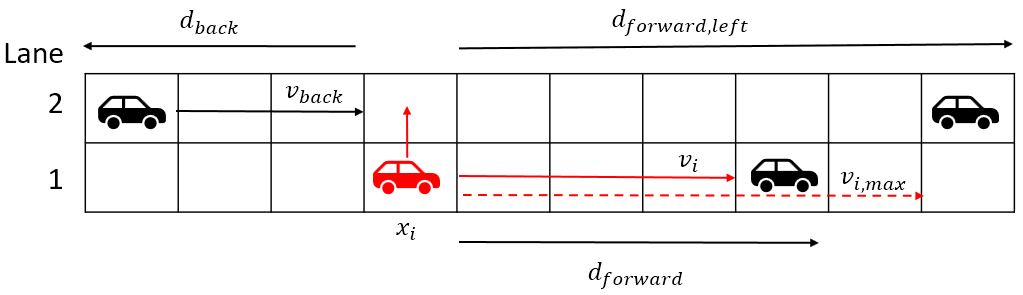
\includegraphics[scale=0.6]{Images/left turn.png}
    \caption{Example of distance calculations for the i:th car marked in red. The car has a desired
    lane change from right to left since $v_i < v_{i, max}$ and $d_{forward,left}>d_{forward}$. The desired lane change
    is allowed since $d_{backward} > v_{back}$.}
    \label{left turn}
\end{figure}

\begin{figure}[H]
    \centering
    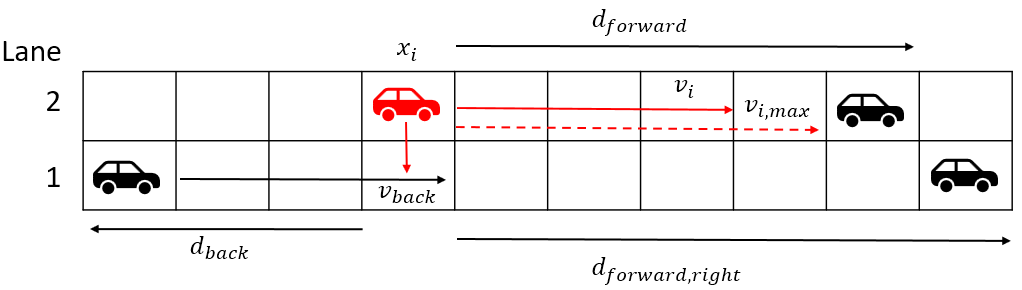
\includegraphics[scale=0.6]{Images/right turn.png}
    \caption{Example of distance calculations for the i:th car marked in red. The car has a desired
    lane change from left to right since $d_{forward} > v_{i, max}$ and $d_{forward_right}>v_{i, max}$. The desired lane change
    is not allowed since $d_{backward} \leq v_{back}$.}
    \label{right turn}
\end{figure}

% diskutera hur diskretiseringen av rum och tid kan påverka!!

\section*{Problem description}
The purpose of this report is to simulate a multi-lane highway and compare how the flow rate is affected by varying the number
of lanes at different car densities.
To do a statistical analysis of the results we would also like to examine the standard error of the flow rate and investigate whether the 
standard error of the flow rate varies depending on the car density and the number of lanes.

\section*{Method}
\subsection*{Setting the system size}
Initially we must choose a system size to run the simulations on where finite size effects can be considered negligible. This is done by plotting fundamental
diagrams of the system while iteratively increasing the road length $L$. When generating the fundamental diagrams the car density is increased by increasing the number
of cars and keeping the road length $L$ constant. This is done separately using 1, 2 and 3 lanes, while keeping remaining system
parameters constant. At a certain road length $L$ the fundamental diagrams will not change as the road length
continues to increase, meaning that the system behavior has become independent of its size. When a road length $L$ is found such that the fundamental diagrams
do not continue to change as $L$ increases the road length will be set to that value for the following simulations.

\subsection*{Flow rate}
To get an understanding of the flow rate behavior and the time necessary to reach equilibrium, the flow rate is plotted against time using a few different 
car densities and the road length $L$ found in the previous section. When the necessary time to reach equilibrium is found, fundamental diagrams are generated using 1, 2 and 3 lanes. Just like previously,
the road length $L$ is always kept constant while generating the fundamental diagrams and only the number of cars is increased. When generating the fundamental diagrams
the flow rate is calculated as an average over 100 time steps after equilibrium has been reached.

\subsection*{Statistical analysis}
In order to examine the statistical accuracy of the results we will study the standard error of the average flow rate after running the simulation multiple times. 
Just like previously, the average flow rate is calculated as an average over 100 time steps after the system has reached equilibrium. Initially, we will examine how the standard error
depends on the number of simulations using a few different car densities. To get a better understanding of the behavior of the standard error the standard error will be calculated
at different car densities using a fixed amount of simulations to get a diagram of how the standard error depends on the car density. This is all done using 1, 2 and 3 lanes separately.

\section*{Results and analysis}
\subsection*{Setting the system size}
The values of $v_{i,max}$ are sampled from a Gaussian distribution with mean $\mu = 10$ and standard deviation $\sigma = 1$. The braking probability
was set to $p=0.2$. The cars are initially placed one unit length ahead of each other evenly distributed in the different lanes according the 
pattern seen in figure \ref*{initial conditions} below.

\begin{figure}[H]
    \centering
    \begin{minipage}{1\textwidth}
        \centering
        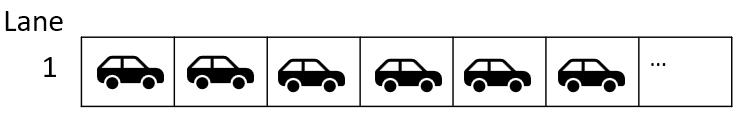
\includegraphics[scale=0.5]{Images/ic 1 lane.png}
        \captionof*{figure}{a) 1 lane}
    \end{minipage}

    \centering
    \begin{minipage}{1\textwidth}
        \centering
        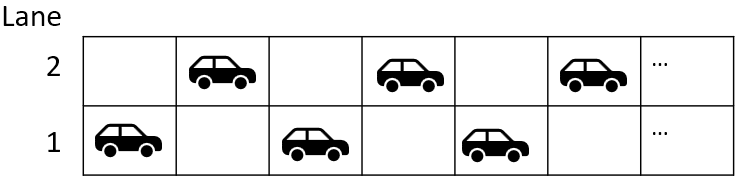
\includegraphics[scale=0.5]{Images/ic 2 lanes.png}
        \captionof*{figure}{b) 2 lanes}
    \end{minipage}

    \centering
    \begin{minipage}{1\textwidth}
        \centering
        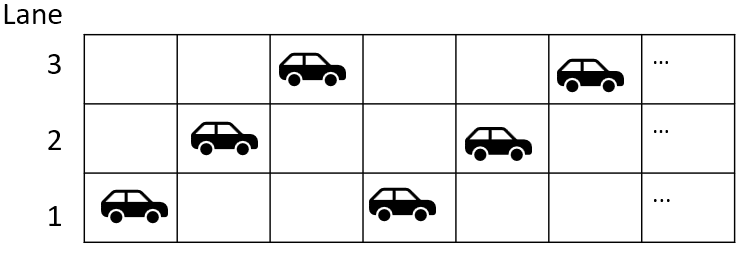
\includegraphics[scale=0.5]{Images/ic 3 lanes.png}
        \captionof*{figure}{c) 3 lanes}
    \end{minipage}%
    \caption{Initial condition of car positions using 1, 2 and 3 lanes.}
    \label{initial conditions}
\end{figure}

Note that these simulation parameters and initial conditions are going to remain unchanged during all following simulations.

Fundamental diagrams are generated by increasing the number of cars $n_{cars}$ so that the car density varies from 0 to 1. 
Each simulation is run for 200 time steps and the flow rate is calculated as an average over the last 100 time steps, as this appears to be 
more than enough to reach equilibrium.
This is done using the different values of the road length $L=20, 40, 60, 80, 100, 120, 140$. In order to reduce random noise in the fundamental diagrams
10 fundamental diagrams are generated for each value of $L$ and a final fundamental diagram is calculated as an average over these 10 fundamental diagrams.
This procedure is done separately using 1, 2 and 3 lanes.
The results can be seen below in figure \ref*{finite size effects}.

\begin{figure}[H]
    \centering
    \begin{minipage}{.5\textwidth}
        \centering
        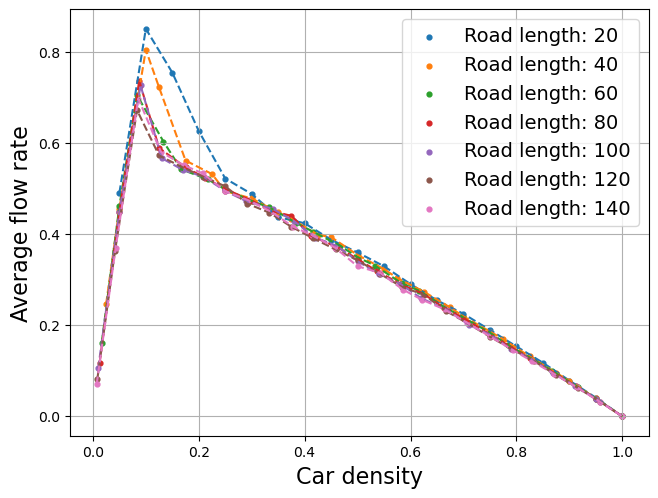
\includegraphics[scale=0.47]{Images/fundamental diagrams 1 lane 140.png}
        \captionof*{figure}{a) 1 lane}
    \end{minipage}%
    \begin{minipage}{.5\textwidth}
        \centering
        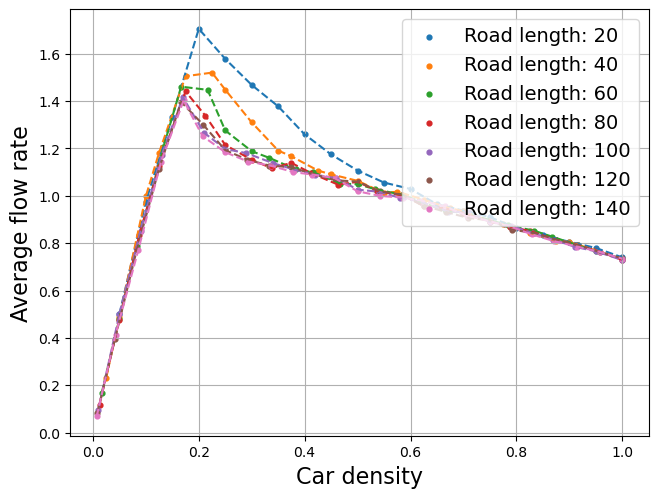
\includegraphics[scale=0.47]{Images/fundamental diagrams 2 lanes 140.png}
        \captionof*{figure}{b) 2 lanes}
    \end{minipage}
    \centering
    \begin{minipage}{.5\textwidth}
        \centering
        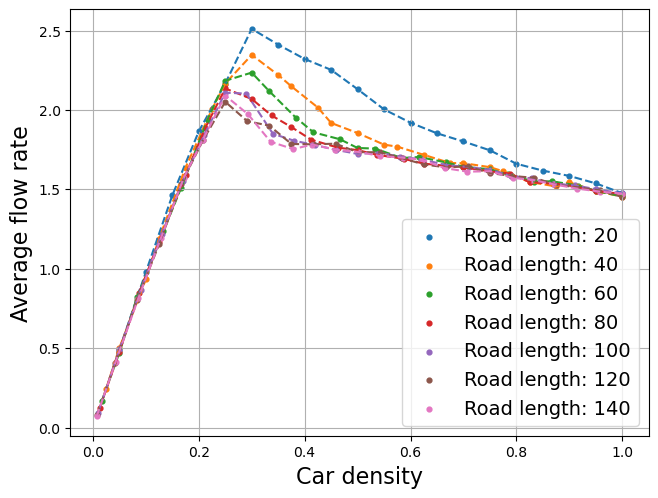
\includegraphics[scale=0.47]{Images/fundamental diagrams 3 lanes 140.png}
        \captionof*{figure}{c) 3 lanes}
    \end{minipage}%
    \caption{Average fundamental diagrams for different road lengths $L$ using 1, 2 and 3 lanes.}
    \label{finite size effects}
\end{figure}

In figure \ref*{finite size effects} we observe that the largest changes in the fundamental diagrams when increasing $L$ occur around the
peak of the fundamental diagrams when the average flow rate is maximal. In figure \ref*{finite size effects} a) when using only 1 lane it appears
as if the system becomes independent of its size at approximately $L=60$, as we can no longer see a change in the fundamental diagrams when increasing
$L$ beyond this value. When increasing the number of lanes a larger value of $L$ appears to be necessary to make the system independent of its size. 
In figure \ref*{finite size effects} b) it appears as if $L=100$ is necessary before the fundamental diagrams stop changing when using 2 lanes. When increasing the number
of lanes to 3 it appears as if $L=120$ is necessary before the fundamental diagrams stop changing, as can be seen in figure \ref*{finite size effects} c).
We thus conclude that a road length of $L=120$ appears to be necessary in order to mitigate finite size effects, and therefore $L=120$ will be used
in following simulations.

\subsection*{Flow rate}
We plot the flow rate over time while using road length $L=120$, and setting the number of cars to $n_{cars}=10, 30, 50$. This is done using 1, 2 and 3 lanes.
The resulting plots of the flow rate against time can be seen below in figure \ref*{flowrate}.
\begin{figure}[H]
    \centering
    \begin{minipage}{.5\textwidth}
        \centering
        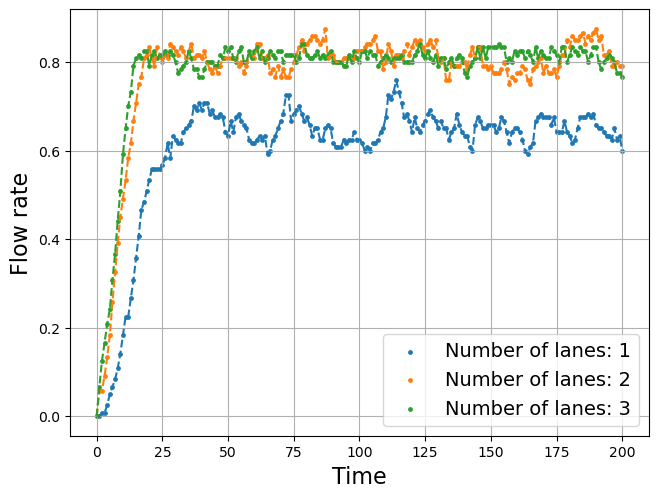
\includegraphics[scale=0.47]{Images/flowrate time 10 cars.png}
        \captionof*{figure}{a) 10 cars}
    \end{minipage}%
    \begin{minipage}{.5\textwidth}
        \centering
        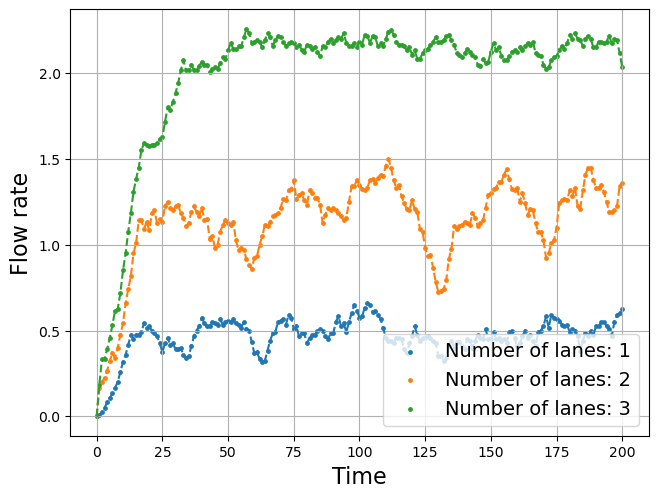
\includegraphics[scale=0.47]{Images/flowrate time 30 cars.png}
        \captionof*{figure}{b) 30 cars}
    \end{minipage}
    \centering
    \begin{minipage}{.5\textwidth}
        \centering
        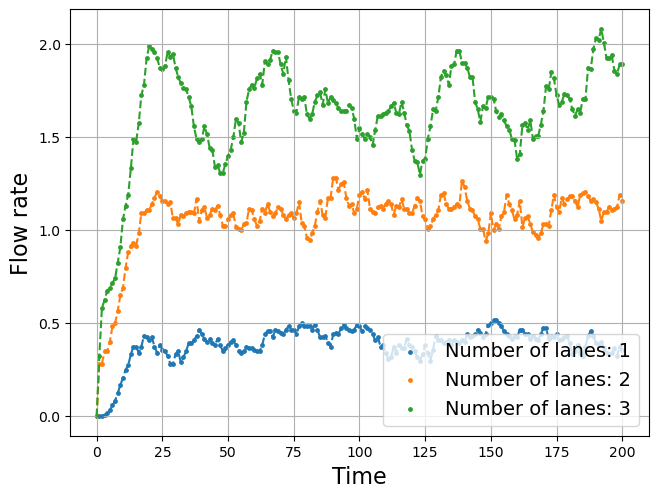
\includegraphics[scale=0.47]{Images/flowrate time 50 cars.png}
        \captionof*{figure}{c) 50 cars}
    \end{minipage}%
    %\begin{minipage}{.5\textwidth}
    %    \centering
    %    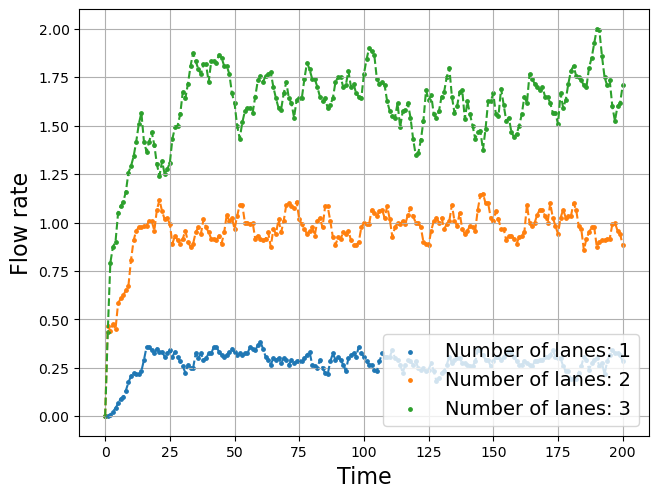
\includegraphics[scale=0.47]{Images/flowrate time 70 cars.png}
    %    \captionof*{figure}{d) 70 cars}
    %\end{minipage}
    \caption{Flow rate plotted against time using different number of cars.}
    \label{flowrate}
\end{figure}
In figure \ref*{flowrate} there appears to be multiple things to note on the flow rate behavior. When $n_{cars}=10$ there is a large gain in the flow rate when increasing
the number of lanes from 1 to 2, while the difference between 2 and 3 lanes is almost none. The fluctuations of the flow rate for the road with 1 lane also
appears to be much larger than when using 2 or 3 lanes. When setting $n_{cars}=30$ we start to see a large gain in the average flow rate when using 3 lanes instead 2.
Interestingly, we also notice that the fluctuations seems to have decreased when using 1 lane and increased when using 2 lanes. 
When further increasing the number of cars to $n_{cars} = 50$ the average gain of the flow rate when increasing the number of lanes
does not appear to change much from before, however the fluctuations are now smaller when using 2 lanes and have significantly increased when using 3 lanes.
It thus appears as if the car density has a large effect on both the average flow rate and the fluctuations of the flow rate.

To get a better understanding of the system dynamics fundamental diagrams are plotted. The flow rate is calculated as an average over the last $100$ time steps when running
the simulation for 200 time steps. The road length $L=120$ is held constant and $n_{cars}$ is iteratively
increased in order to increase the car density from 0 to 1. The results are seen below in figure \ref*{fundamental diagram}.

\begin{figure}[H]
    \centering
    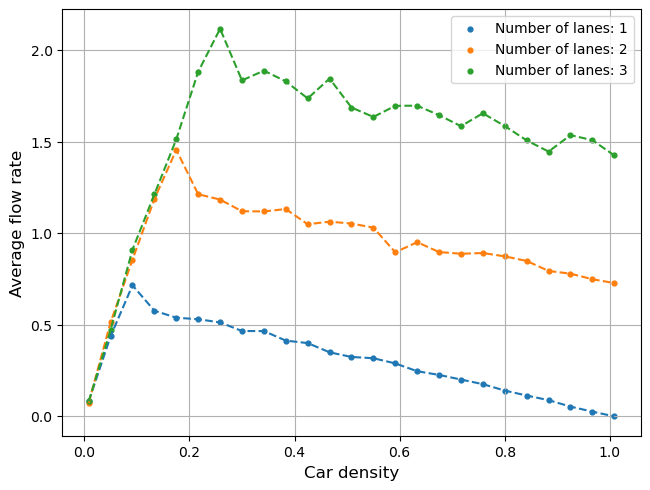
\includegraphics[scale=0.9]{Images/fundamental diagram 120.png}
    \caption{Average flow rate plotted against car density for different number of lanes.}
    \label{fundamental diagram}
\end{figure}

In figure \ref*{fundamental diagram} we see that the flow rate appears to grow linearly until a clear maximum value is reached. When increasing the car density beyond
that value the flow rate appears to decrease, also somewhat linearly. For low car densities the average flow rate appears independent of the number of lanes.
This is reasonable since we should not be expecting a gain in the flow rate by having a large amount of lanes when very few cars are on the road.
The car density required in order to reach the maximum value of the average flow rate appears to increase when the number of lanes increase. Interestingly, both the positive derivate
of the flow rate before the maximum value has been reached, and the negative derivate of the flow rate after the maximum value has been reached appear to be equal for all
number of lanes. 

We can also note that the gain in the flow rate acquired by increasing the number of lanes appears to be the same when increasing the number of lanes from 1 to 2 as when
increasing the number of lanes from 2 to 3, given that the car density is larger than approximately 0.25 (where the flow rate using 3 lanes reaches its maximum value).
For lower car densities the gain in the flow rate acquired by increasing the number of lanes depends on the car density.

\subsection*{Statistical accuracy}
We will now examine the statistical accuracy by calculating the standard error of the average flow rate. Just like in the previous section we initially run the simulation
using $n_{cars}=10, 30, 50$. Simulations are run for 200 time steps and the flow rate is calculated as an average over the last 100 time steps.
We run the simulations multiple times and calculate the standard error of the flow rate values using 1, 2 and 3 lanes. Diagrams showing the
standard error of the flow rate plotted against the number of simulations are seen below in figure \ref*{standard error 1}.

\begin{figure}[H]
    \centering
    \begin{minipage}{.5\textwidth}
        \centering
        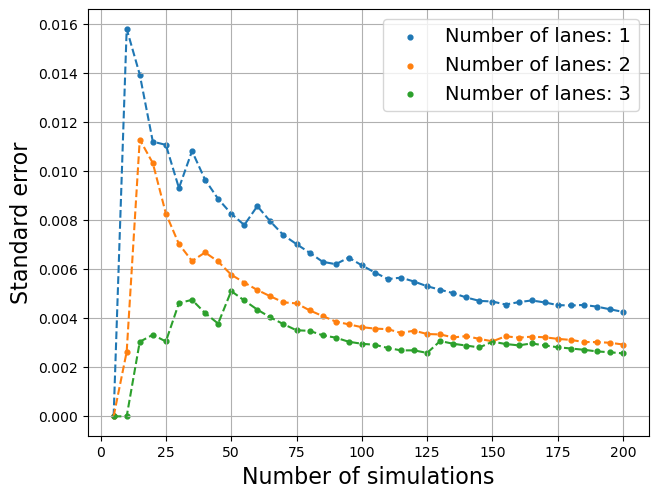
\includegraphics[scale=0.47]{Images/standard error 10 cars 120.png}
        \captionof*{figure}{a) 10 cars}
    \end{minipage}%
    \begin{minipage}{.5\textwidth}
        \centering
        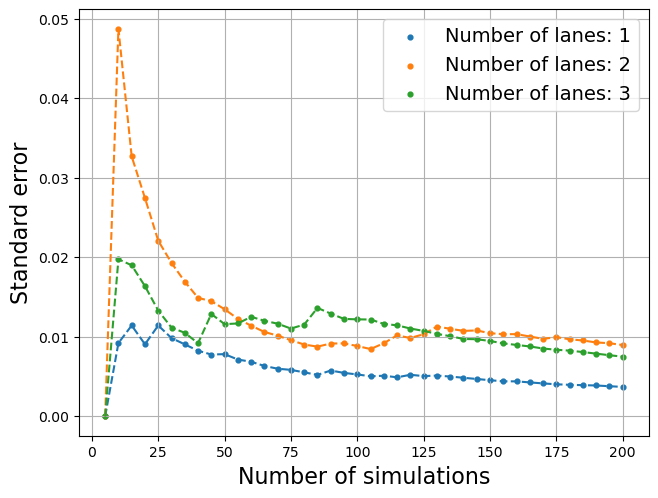
\includegraphics[scale=0.47]{Images/standard error 30 cars 120.png}
        \captionof*{figure}{b) 30 cars}
    \end{minipage}
    \centering
    \begin{minipage}{.5\textwidth}
        \centering
        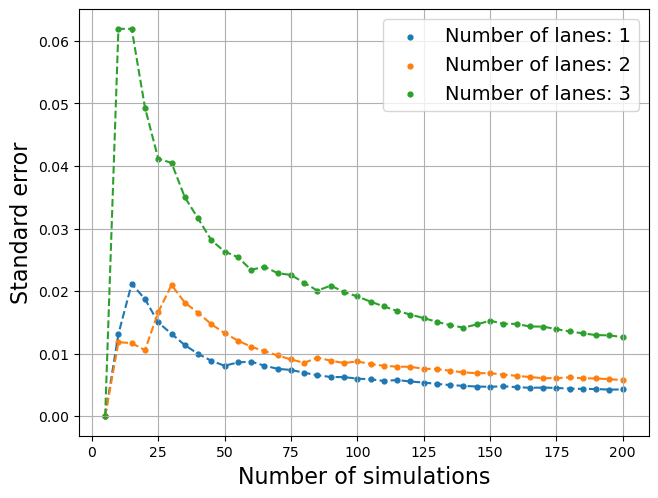
\includegraphics[scale=0.47]{Images/standard error 50 cars 120.png}
        \captionof*{figure}{c) 50 cars}
    \end{minipage}%
    %\begin{minipage}{.5\textwidth}
    %    \centering
    %    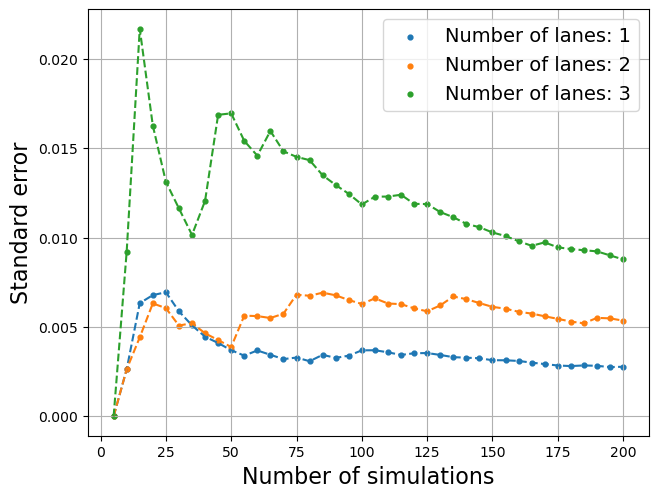
\includegraphics[scale=0.47]{Images/standard error 70 cars 120.png}
    %    \captionof*{figure}{d) 70 cars}
    %\end{minipage}
    \caption{Standard error of average flow rate plotted against amount of simulations using different number of cars and lanes.}
    \label{standard error 1}
\end{figure}

When using $n_{cars}=10$ it is clear that the standard error of the flow rate is much larger when using 1 lane compared to 2 or 3 lanes.
When $n_{cars}=30$ the standard error is the largest when using 2 lanes and the standard error when using 1 lane appears to have decreased.
Setting the number of cars to $n_{cars}=50$ we instead see the highest standard error when using 3 lanes and lower standard error than before 
when using 2 lanes. These large differences in the standard error depending on the number of lanes and the car density appear to 
be consistent with the results seen in figure \ref*{flowrate} in the previous section.

To get a better understanding of how the standard error depends on the car density we calculate the standard error for varying car densities.
The road length remains fixed at $L=120$ and the number of cars is iteratively increased in order to vary the car density from 0 to 1. For each car density 100 simulations are run
for 200 time steps. The flow rate is calculated as an average over the last 100 time steps. The standard error of the flow rate values is then calculated.
This is done using 1, 2 and 3 lanes. The results can be seen below in figure \ref*{standard error}.

\begin{figure}[H]
    \centering
    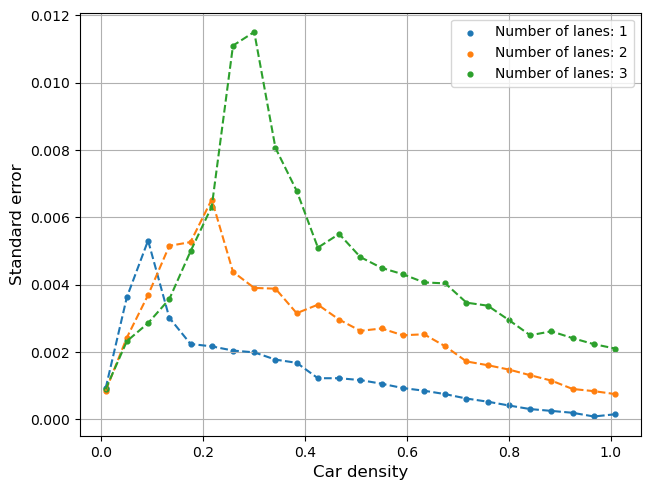
\includegraphics[scale=0.9]{Images/standard error 120.png}
    \caption{Standard error of average flow rate plotted against car density for different number of lanes.}
    \label{standard error}
\end{figure}

In figure \ref*{standard error} we notice that the plots of the standard error against the car density are somewhat similar to the fundamental diagrams
in figure \ref*{fundamental diagram}. For all number of lanes, we initially see a clear increase of the standard error as the car density increases
until a clear peak value is reached. Increasing the car density further makes the standard error decrease. When comparing the different number of lanes we primarily
see two main differences. Firstly, we notice that the car density for which the standard error reaches its maximum value is larger when increasing the number of lanes.
Secondly, we notice that the maximum value of the standard error increases when increasing the number of lanes. If we compare figure \ref*{standard error} with the fundamental
diagrams in figure \ref*{fundamental diagram} it appears as if the car densities for which the flow rates reach their maximum
values are very similar to the car densities for which the standard errors reach their maximum values. These results will be analyzed further in the discussion.

\section*{Discussion}
\subsection*{Model discussion}
In order to construct the model used in this report several assumptions have been made. For example, the drivers have been assumed to be skilled
since a car will never perform a lane change if that means that a car behind will have to brake. In order to better model the varying
driving skill of real life drivers, the model could possibly be modified in order to allow some lane changes even when that means other 
cars will have to slow down.

Furthermore, we have assumed the distribution of driver preferred maximum speed (i.e. the values of $v_{i,max})$ to be Gaussian distributed, with the same mean $\mu$ and standard
deviation $\sigma$ regardless of car density.
The model could possibly be improved by developing a more sophisticated model of the distribution of desired maximum speed.

Another important aspect to mention are the possible consequences of using period boundary conditions. When using period boundary conditions there is a risk
that a car might detect itself as the car in front. The car would then calculate the periodic distance to itself and adjust its speed accordingly. 
This is highly unrealistic and something we must be aware of when using period boundary conditions. This problem and other finite size effects are most
likely mitigated when the system size is set such that the system becomes independent of its size.

\subsection*{Results discussion}
When analyzing the fundamental diagrams in figure \ref*{fundamental diagram} a few key conclusions can be made.
Mainly, we can see that a higher car density is required to maximize the flow rate when using more lanes and that
the maximum flow rate is also higher when using more lanes. These results are in no way surprising, however still serve
as a good confirmation that the chosen model is able to produce somewhat realistic results. 

We can also note that before the fundamental diagrams for the different number of lanes had reached their maximum values the positive derivate of the flow rate appeared to be the same
regardless of the number of lanes used.
This was also true after all fundamental diagrams had reached their maximum value, as we could then see all the negative derivates of the flow rate also being approximately the same.
This fact is less obvious and without analyzing real traffic data it is hard to determine whether this pattern is something that would occur in real traffic flow or if it is simply
a result of the simplified model. 

The most interesting results however appear during the statistical analysis of the results.
According to the results seen in figure \ref*{fundamental diagram} and figure \ref*{standard error} the car density for which the flow rate reaches its maximum value appears
to be the same as the car density for which the flow rate standard error reaches its maximum value. The model results thus indicate that it might be impossible to maximize the flow rate while still
achieving low fluctuations of the flow rate (assuming that the standard error is a good way to measure the amount of fluctuations). These results appear quite reasonable since when the flow rate is maximal it is logical that the system would be more sensitive
to small perturbations since there is a lot of activity on the road. If the model is correct, there would thus be a clear trade off between having a high flow rate and
low fluctuations of the flow rate when planning road infrastructure.
Furthermore, one would have to be especially careful when increasing the number of lanes at high car densities, 
as this appeared to significantly increase the fluctuations of the flow rate, as seen in figure \ref*{standard error}.

In order to determine if the model results actually hold in real traffic flow, real traffic data would have to be analyzed and compared to the model results.

\end{document}